% !TEX root =  ../supplementary.tex
\section{Personalized Biopsies Based on Cause-Specific Cumulative Upgrading-Risk}
Consider some real patients from the PRIAS database shown in Figure~\ref{fig:demo_pat1_supp}--~\ref{fig:demo_pat3_supp}. We intend to develop personalized schedule of biopsies for these patients. Using the joint model fitted to the PRIAS dataset, we first obtain their cause-specific cumulative upgrading-risk over the entire follow-up period (see Equation~\ref{eq:dynamic_risk_prob}), given their accumulated clinical data. Our aim is to employ this cumulative-risk function in the personalized biopsy schedule. However, in line with the protocols of most AS cohorts~\citep{nieboer2018active}, we first schedule a compulsory biopsy at year one of follow-up. This promises early detection of Gleason upgrade for patients misdiagnosed as low-grade cancer patients, or patients who chose AS despite having a higher grade at diagnosis. We also maintain a recommended minimum gap of one year between consecutive biopsies~\citep{bokhorst2015compliance}. Consequently, we schedule personalized biopsies starting from year two until year a maximum horizon (Table~\ref{tab:max_pred_time_repeat}). The added benefit of this approach is that due to the longitudinal measurements accumulated over two years, and year one biopsy results, we are able to make reasonably accurate predictions of the cause-specific cumulative upgrading-risk. 

We next exploit PRIAS cohort's fixed schedule of longitudinal measurements ${L=\{2, 2.5 \ldots 6\}}$ between year two and six (horizon, Table~\ref{tab:max_pred_time_repeat}). More specifically, we schedule a biopsy at all those future visits where the conditional cause-specific cumulative upgrading-risk is larger than a certain threshold $0 \leq \kappa \leq 1$ (e.g., 10\% risk). The resulting personalized schedule of biopsies $B_j^{\kappa}$ is given by:
\begin{equation}
\label{eq:personalized_schedule}
\begin{split}
B_j^{\kappa} &= \Big\{b_{jk} \epsilon L \mid R_j(b_{jk} \mid b_{jk-1}, s) \geq \kappa \land (b_{jk}-b_{jk-1}\geq 1) \Big\},
\end{split}
\end{equation}
where $b_{jk}$ is the time of the $k$-th biopsy for the $j$-th patient and $b_{j0}$ corresponds to time of the last conducted biopsy before making this schedule. The conditional cause-specific cumulative upgrading-risk denoted by $R_j(b_{jk} \mid b_{jk-1}, s)$ is defined as in Equation~(\ref{eq:dynamic_risk_prob}). In this risk the contribution of the observed PSA $\mathcal{Y}_{j}(s)$ does not change while scheduling subsequent biopsies. However, the `conditional' part here is that successive $k$-th biopsy at time $b_{jk}$ is scheduled by accounting for the possibility that Gleason upgrade may not have occurred until the previously scheduled biopsy $T^*_j > b_{jk-1}$. The personalized schedule Equation~(\ref{eq:personalized_schedule}) is updated as more patient data becomes available over follow-up.

\begin{table}[!htb]
\small\sf\centering
\caption{\textbf{Maximum follow-up period up to which we can reliably make personalized schedules}. In each cohort, this time point is chosen such that there are at least 10 patients who experience upgrading after this time point. Full names of Cohorts are \textit{PRIAS}: Prostate Cancer International Active Surveillance, \textit{Toronto}: University of Toronto Active Surveillance, \textit{Hopkins}: Johns Hopkins Active Surveillance, \textit{MSKCC}: Memorial Sloan Kettering Cancer Center Active Surveillance, \textit{KCL}: King's College London Active Surveillance, \textit{MUSIC}: Michigan Urological Surgery Improvement Collaborative Active Surveillance, \textit{UCSF}: University of California San Francisco Active Surveillance.}
\label{tab:max_pred_time_repeat}
\begin{tabular}{l|r}
\hline
\hline
Cohort & \parbox[t]{3.75cm}{Maximum Personalized\\Schedule Time (years)}\\
\hline
PRIAS & 6\\
KCL & 3\\
MUSIC & 2\\
Toronto & 8\\
MSKCC & 6\\
Hopkins & 7\\
UCSF & 8.5\\
\hline
\end{tabular}	
\end{table}

To assist patients in making an informed choice for a schedule, be it personalized or fixed, we provide them patient-specific consequences of following each schedule. To this end, we first calculate the probability of occurrence of upgrading between successive biopsies of each schedule. Using these probabilities we then obtain the expected delay in detection of upgrading for following that schedule. Thus, patients have a method to compare across various schedules in terms of the personalized burden (time and total biopsies), and personalized benefit (less delay in detection of upgrading is beneficial). Suppose once again that for patient $j$, the time of latest negative biopsy is $t$, and current visit time is $s > t$. Then equation for the expected delay $D_j(B \mid t,s)$ in detection of upgrading using schedule of biopsies $B = \{b_1, \ldots, b_h\}$, where $b_1 \geq s$, and $b_h$ is the horizon time (Table~\ref{tab:max_pred_time_repeat}) up to which we want to schedule biopsies, is given by:
\begin{equation}
\label{eq:expected_delay}
\begin{split}
D_j(B \mid t,s) &= \sum_{v=1}^{h} R_j(b_v\mid b_{v-1},s) \times  \Big\{b_{v} - b_{v-1} - \int_{b_{v-1}}^{b_v} S_j(u \mid b_v, b_{v-1}, s) \mathrm{d}u \Big\},\\
S_j(u \mid b_v, b_{v-1}, s) &= \mbox{Pr}\big\{T^*_j > u \mid b_{v} \geq T^*_j > b_{v-1}, \mathcal{Y}_{j}(s), \mathcal{D}_n\big\}, \quad b_{v} \geq u > b_{v-1},
\end{split}
\end{equation}
and $R_j(b_v\mid b_{v-1},s)$ is as defined in Equation~(\ref{eq:dynamic_risk_prob}). The personalized and fixed schedules, and their consequences for a few real patients from the PRIAS dataset are shown in Figure~\ref{fig:demo_pat1_supp} to Figure~\ref{fig:demo_pat3_supp}. A compulsory biopsy was done at horizon $b_h$ of follow-up in all schedules for meaningful comparison of their expected delays in detection of upgrading.

\begin{figure}
\centerline{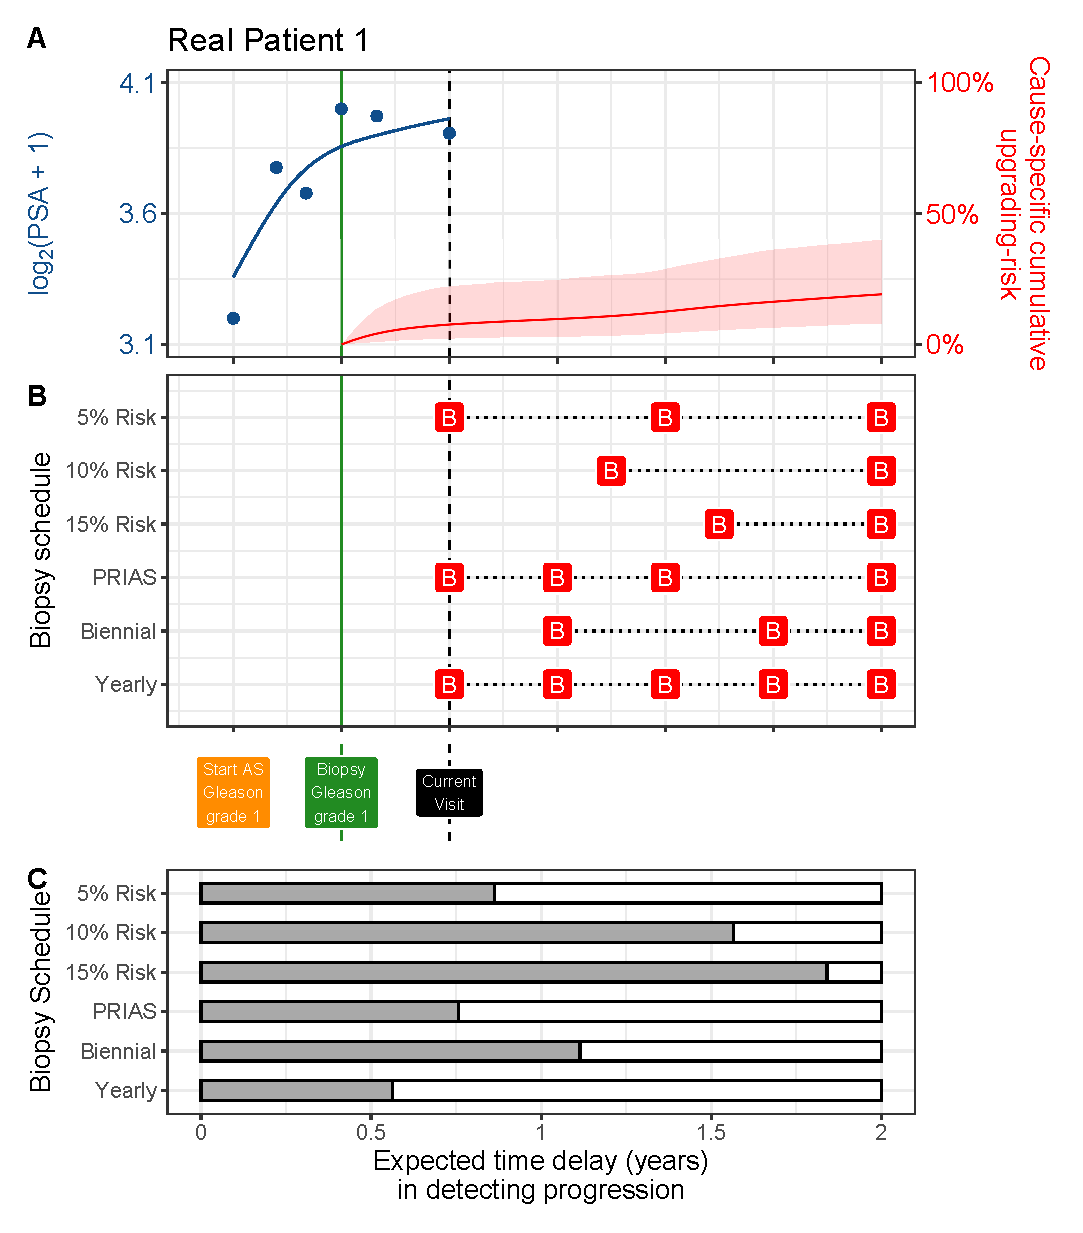
\includegraphics[width=\columnwidth]{images/demo_pat1_supp.eps}}
\caption{\textbf{Personalized and fixed schedules of biopsies for patient 1}. \textbf{Panel~A:} shows the observed and fitted $\log_2(\mbox{PSA} + 1)$ measurements (Equation~\ref{eq:long_model_psa}), and the dynamic cause-specific cumulative upgrading-risk (see \ref{sec:param_estimates_jm_fit_prias}) over follow-up period. \textbf{Panel~B} shows the personalized and fixed schedules of biopsies with a `B' indicating times of biopsies. \textbf{Panel~B} various schedules are compared in terms of the expected delay in detection of upgrading if they are followed. A compulsory biopsy was scheduled at year six (maximum biopsy scheduling time in PRIAS, Supplementary~C) in all schedules for a meaningful comparison between them.}
\label{fig:demo_pat1_supp}
\end{figure}

\begin{figure}
\centerline{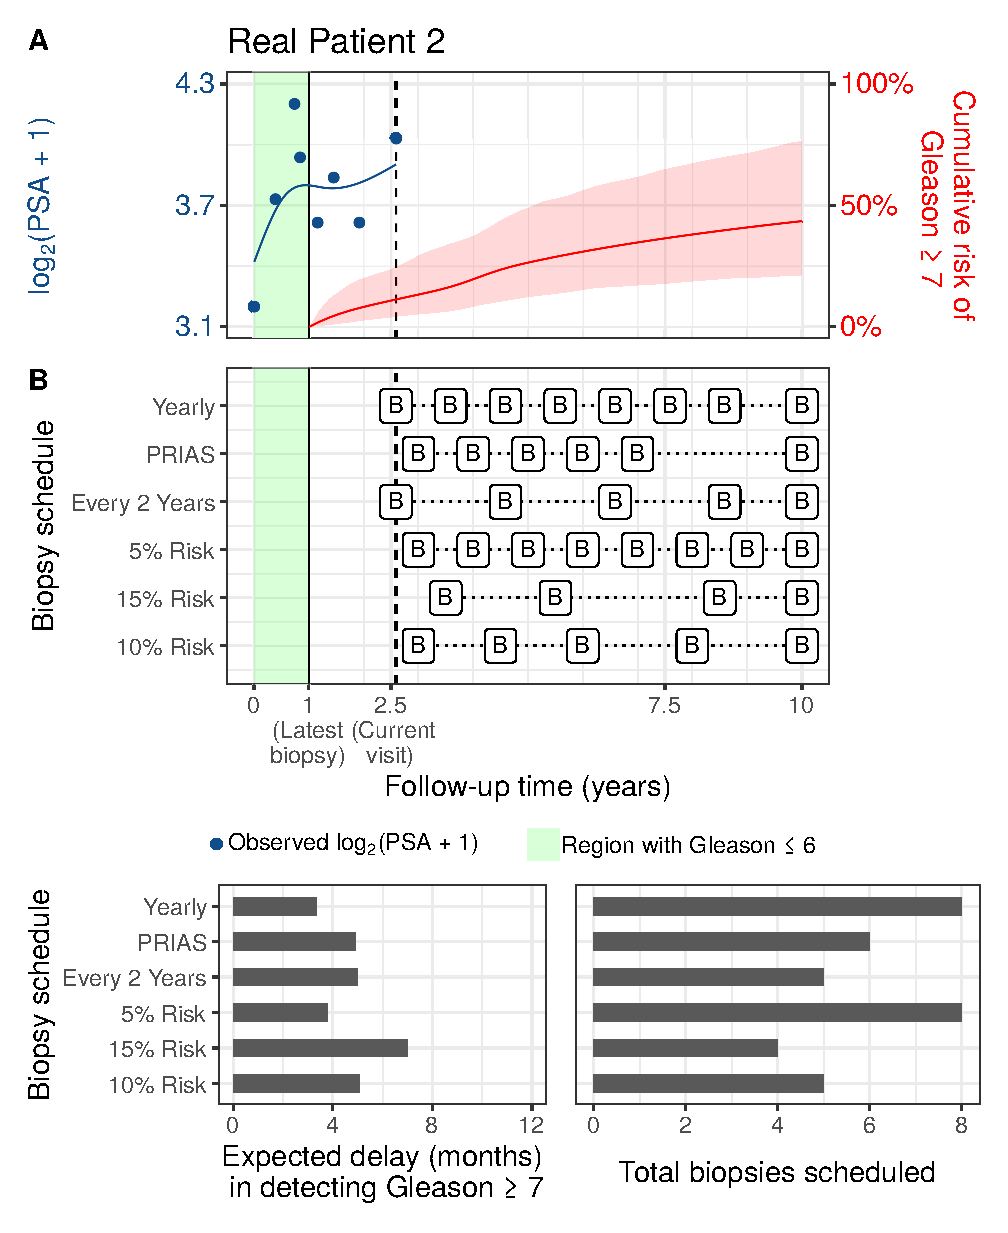
\includegraphics[width=\columnwidth]{images/demo_pat2_supp.eps}}
\caption{\textbf{Personalized and fixed schedules of biopsies for patient 2}. \textbf{Panel~A:} shows the observed and fitted $\log_2(\mbox{PSA} + 1)$ measurements (Equation~\ref{eq:long_model_psa}), and the dynamic cause-specific cumulative upgrading-risk (see \ref{sec:param_estimates_jm_fit_prias}) over follow-up period. \textbf{Panel~B} shows the personalized and fixed schedules of biopsies with a `B' indicating times of biopsies. \textbf{Panel~B} various schedules are compared in terms of the expected delay in detection of upgrading if they are followed. A compulsory biopsy was scheduled at year six (maximum biopsy scheduling time in PRIAS, Supplementary~C) in all schedules for a meaningful comparison between them.}
\label{fig:demo_pat2_supp}
\end{figure}

\begin{figure}
\centerline{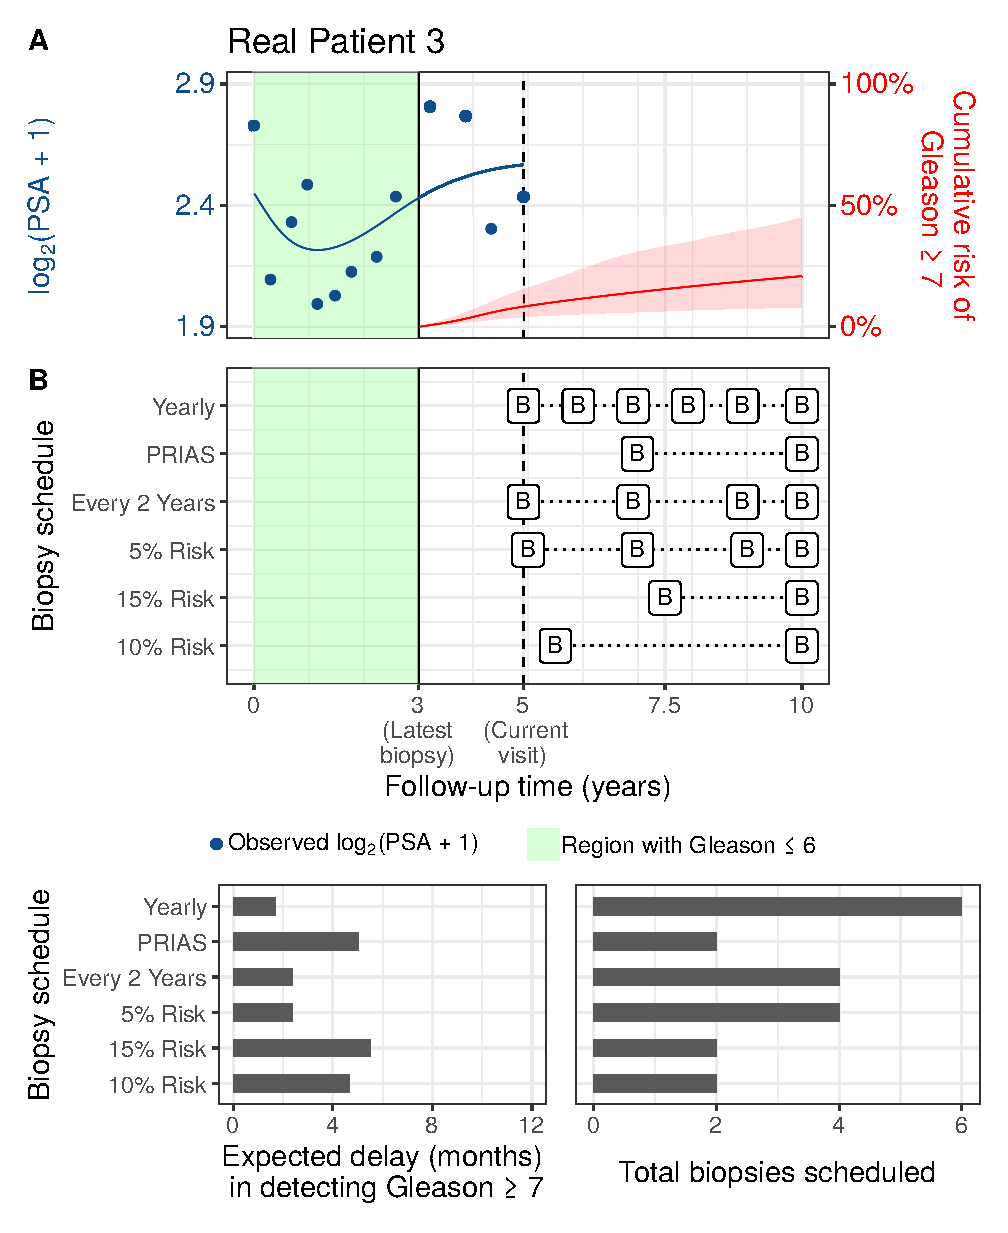
\includegraphics[width=\columnwidth]{images/demo_pat3_supp.eps}}
\caption{\textbf{Personalized and fixed schedules of biopsies for patient 3}. \textbf{Panel~A:} shows the observed and fitted $\log_2(\mbox{PSA} + 1)$ measurements (Equation~\ref{eq:long_model_psa}), and the dynamic cause-specific cumulative upgrading-risk (see \ref{sec:param_estimates_jm_fit_prias}) over follow-up period. \textbf{Panel~B} shows the personalized and fixed schedules of biopsies with a `B' indicating times of biopsies. \textbf{Panel~B} various schedules are compared in terms of the expected delay in detection of upgrading if they are followed. A compulsory biopsy was scheduled at year six (maximum biopsy scheduling time in PRIAS, Supplementary~C) in all schedules for a meaningful comparison between them.}
\label{fig:demo_pat3_supp}
\end{figure}